\documentclass[12pt]{book}

\newcommand{\thetitle}{Think Java: How to Think Like a Computer Scientist}
\title{\thetitle}

\newcommand{\theauthors}{Allen Downey and Chris Mayfield}
\author{\theauthors}

\newcommand{\theversion}{Version 6.0 Draft -- \today}
\date{\theversion}

\usepackage{geometry}
\geometry{
    width=5.5in,
    height=8.5in,
    hmarginratio=3:2,
    vmarginratio=1:1,
    includehead=true,
    headheight=15pt
}

% paragraph spacing
\setlength{\parindent}{0pt}                      % 17.62482pt
\setlength{\parskip}{12pt plus 4pt minus 4pt}    % 0.0pt plus 1.0pt
\linespread{1.05}
\def\arraystretch{1.5}

% list spacing
\setlength{\topsep}{5pt plus 2pt minus 3pt}      % 10.0pt plus 4.0pt minus 6.0pt
\setlength{\partopsep}{-6pt plus 2pt minus 2pt}  %  3.0pt plus 2.0pt minus 2.0pt
\setlength{\itemsep}{0pt}                        %  5.0pt plus 2.5pt minus 1.0pt

% these are copied from tex/latex/base/book.cls
% all I changed is afterskip
\makeatletter
\renewcommand{\section}{\@startsection {section}{1}{\z@}%
    {-3.5ex \@plus -1ex \@minus -.2ex}%
    {0.7ex \@plus.2ex}%
    {\normalfont\Large\bfseries}}
\renewcommand\subsection{\@startsection{subsection}{2}{\z@}%
    {-3.25ex\@plus -1ex \@minus -.2ex}%
    {0.3ex \@plus .2ex}%
    {\normalfont\large\bfseries}}
\renewcommand\subsubsection{\@startsection{subsubsection}{3}{\z@}%
    {-3.25ex\@plus -1ex \@minus -.2ex}%
    {0.3ex \@plus .2ex}%
    {\normalfont\normalsize\bfseries}}
\makeatother

% table of contents vertical spacing
\usepackage{tocloft}
\setlength\cftparskip{8pt plus 4pt minus 4pt}

% The following line adds a little extra space to the column
% in which the Section numbers appear in the table of contents
\makeatletter
\renewcommand{\l@section}{\@dottedtocline{1}{1.5em}{3.0em}}
\makeatother

% customize page headers
\usepackage{fancyhdr}
\pagestyle{fancyplain}
\renewcommand{\chaptermark}[1]{\markboth{Chapter \thechapter ~~ #1}{}}
\renewcommand{\sectionmark}[1]{\markright{\thesection ~~ #1}}
\lhead[\fancyplain{}{\bfseries\thepage}]%
      {\fancyplain{}{\bfseries\rightmark}}
\rhead[\fancyplain{}{\bfseries\leftmark}]%
      {\fancyplain{}{\bfseries\thepage}}
\cfoot{}
%\rfoot{\textcolor{gray}{\tiny ThinkJava Draft \today}}

% balanced index with TOC entry
\usepackage{makeidx}
\makeindex
%\usepackage[totoc]{idxlayout}

% automatically index glossary terms
\newcommand{\term}[1]{%
\index{#1}
\item[#1:]}
% TODO: doesn't work with plastex
%\newcommand{\term}[1]{\item[#1:]}

% where to find graphics
\usepackage{graphicx}
%\graphicspath{{figs/}}

%% tweak spacing of figures and captions
%\usepackage{floatrow}
%\usepackage{caption}
%\captionsetup{
%    font=small,
%    labelformat=empty,
%    justification=centering,
%    skip=4pt
%}

% format end of chapter excercises
\usepackage{amsmath}
\usepackage{amsthm}
\newtheoremstyle{exercise}
  {12pt}        % space above
  {12pt}        % space below
  {}            % body font
  {}            % indent amount
  {\bfseries}   % head font
  {}            % punctuation
  {12pt}        % head space
  {}            % custom head
\theoremstyle{exercise}
\newtheorem{exercise}{Exercise}[chapter]

% colors for code listings and output
\usepackage{xcolor}
\definecolor{bgcolor}{HTML}{FAFAFA}
\definecolor{comment}{HTML}{007C00}
\definecolor{keyword}{HTML}{0000FF}
\definecolor{strings}{HTML}{B20000}

% syntax highlighting in code listings
\usepackage{textcomp}
\usepackage{listings}
\lstset{
    language=java,
    basicstyle=\ttfamily,
    backgroundcolor=\color{bgcolor},
    commentstyle=\color{comment},
    keywordstyle=\color{keyword},
    stringstyle=\color{strings},
    columns=fullflexible,
    keepspaces=true,
    showstringspaces=false,
    upquote=true,
    aboveskip=\parskip,
    belowskip=\parskip
}

% code listing environments
\lstnewenvironment{code}
{\minipage{\linewidth}}
{\endminipage}
\lstnewenvironment{stdout}
{\lstset{commentstyle=,keywordstyle=,stringstyle=}\minipage{\linewidth}}
{\endminipage}

% pdf hyperlinks, table of contents, and document properties
\usepackage[pdftex]{hyperref}
\hypersetup{%
  pdftitle={\thetitle},
  pdfauthor={\theauthors},
  pdfsubject={\theversion},
  pdfkeywords={},
  bookmarksopen=false,
  colorlinks=true,
  citecolor=black,
  filecolor=black,
  linkcolor=black,
  urlcolor=blue
}

% inline syntax formatting
\newcommand{\java}[1]{\lstinline{#1}} %\end{
%\newcommand{\java}[1]{\verb"#1"}
%\newcommand{\java}[1]{{\tt #1}}

\begin{document}
\setcounter{chapter}{10}


\chapter{Arrays of integers}
\label{arrays}

\index{array}
\index{type!array}

An {\bf array} is a set of values where each value is identified by an index.
You can make an array of \java{int}s, \java{double}s, or any other type, but all the values in an array must have the same type.

Syntactically, array types look like other Java types except they are followed by square brackets \java{[]}.
For example, \java{int[]} is the type ``integer array'' and \java{double[]} is the type ``double array.''

You can declare variables with these types in the usual way:

\begin{code}
    int[] counts;
    double[] values;
\end{code}

Arrays are objects and must be created.
An array variable simply stores a reference to an array object.
To create the array itself, use the \java{new} operator.

\begin{code}
    counts = new int[4];
    values = new double[size];
\end{code}

The first assignment makes \java{count} refer to an array of 4 integers.
The second makes \java{values} refer to an array of \java{double}s, but the number of elements in \java{values} depends on the variable \java{size}.
You can use any integer expression for the size of an array.

\section{Accessing elements}

\index{memory diagram}

When you allocate an array of \java{int}s, the elements are automatically initialized to zero.
Here is a memory diagram of the \java{counts} array so far:

\begin{center}
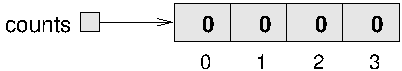
\includegraphics{figs/array.pdf}
\end{center}

\index{element}
\index{index}
\index{array!element}
\index{array!index}

The large numbers inside the boxes are the {\bf elements} of the array.
The small numbers outside the boxes are the {\bf indexes} (or indices) used to identify each memory location.

To store values in the array, use the \java{[]} operator.
For example \java{counts[0]} refers to the ``zeroeth'' element of the array, and \java{counts[1]} refers to the ``oneth'' element.  You can use the \java{[]} operator anywhere in an expression:

\begin{code}
    counts[0] = 7;
    counts[1] = counts[0] * 2;
    counts[2]++;
    counts[3] -= 60;
\end{code}

These assignment statements are all legal in Java.
Here is the result of the above code fragment:

\begin{center}
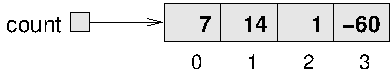
\includegraphics{figs/array2.pdf}
\end{center}

\index{exception!ArrayOutOfBounds}
\index{run-time error}

The elements of the array are numbered from 0 to 3, which means that there is no element with the index 4.
This should sound familiar, since we saw the same thing with \java{String} indexes.
Nevertheless a common programming mistake is going beyond the bounds of an array, which throws an \java{ArrayIndexOutOfBoundsException}.

You can use any expression as an index, as long as it has type \java{int}.
One of the most common ways to index an array is with a loop variable.
For example:

\begin{code}
    int i = 0;
    while (i < 4) {
        System.out.println(counts[i]);
        i++;
    }
\end{code}

\index{loop}
\index{loop variable}
\index{variable!loop}

This is a standard \java{while} loop that counts from 0 up to 4.
When the loop variable \java{i} is 4, the condition fails and the loop terminates.
Thus, the body of the loop is only executed when \java{i} is 0, 1, 2 and 3.

Each time through the loop we use \java{i} as an {\it index} into the array, printing the \java{i}th element.
For convenience, this type of array traversal is commonly written using a \java{for} loop.

\begin{code}
    for (int i = 0; i < 4; i++) {
        System.out.println(counts[i]);
    }
\end{code}

%\section{Arrays vs objects}

\index{object!compared to array}
\index{array!compared to object}

Some of the objects we looked at, like \java{Rectangle}s, are similar to arrays in the sense that they are a set of values.
Because arrays are also objects, they have many of the same behaviors:

\begin{itemize}

\item When you declare an array variable, you get a reference to an array.

\item You have to use \java{new} to create the array itself.

\item When you pass an array as an argument, you pass a reference, which means that the invoked method can change the contents of the array.

\end{itemize}

You might ask, ``How is an array of 4 integers different from a Rectangle object of 4 integers?''
The main difference is that array elements are accessed by index, whereas object elements have names.
Another difference is that the elements of an array have to be the same type; objects can have instance variables with different types.


\section{Copying arrays}
\index{array!copying}

When you copy an array variable, remember that you are copying a reference to the array.
For example:

\begin{code}
    double[] a = new double[3];
    double[] b = a;
\end{code}

This code creates one array of three \java{double}s and sets two different variables to reference it.
As with objects, this situation is a form of aliasing.

\begin{center}
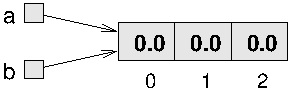
\includegraphics{figs/array3.pdf}
\end{center}

Any changes made through either array variable will be reflected in the other.
This behavior is usually not what you want; more often you want to allocate a \java{new} array and copy elements from one to the other.

\begin{code}
    double[] b = new double[3];
    for (int i = 0; i < 3; i++) {
        b[i] = a[i];
    }

\end{code}

\index{java.util.Arrays}

The Java library provides a utility class named \java{java.util.Arrays} with methods for copying arrays and other common array operations.
We can rewrite the above \java{for} loop with just one line of code.

\begin{code}
    double[] b = Arrays.copyOf(a, 3);
\end{code}

%\section{Array length}

\index{length!array}
\index{array!length}

All arrays have one named instance variable: \java{length}.
Not surprisingly, it contains the length of the array (number of elements).
It is a good idea to use this value as the upper bound of a loop, rather than a constant value.
That way, if you need to change the size of the array, you won't have to go through the program changing all the loops.

\begin{code}
    for (int i = 0; i < a.length; i++) {
        b[i] = a[i];
    }
\end{code}

The last time the body of the loop gets executed, \java{i} is \java{a.length - 1}, which is the index of the last element.
When \java{i} is equal to \java{a.length}, the condition fails and the body is not executed (which is a good thing, since it would throw an exception).

The above \java{for} loop assumes that the array \java{b} contains at least as many elements as \java{a}.
Of course, you could simply use the \java{Arrays} class and \java{a.length}:

\begin{code}
    b = Arrays.copyOf(a, a.length);
\end{code}


\section{Random numbers}
\label{random}
\label{pseudorandom}

\index{deterministic}

Most computer programs do the same thing every time they are executed, so they are said to be {\bf deterministic}.
Usually determinism is a good thing, since we expect the same calculation to yield the same result.
But for some applications we want the computer to be unpredictable.
Games are an obvious example, but there are many others.

\index{nondeterministic}

Making a program truly {\bf nondeterministic} turns out to be not so easy, but there are ways to make it at least seem nondeterministic.
One of them is to generate random numbers and use them to determine the outcome of the program.
Java provides a method that generates {\bf pseudorandom} numbers, which are not truly random since they are determined by an algorithm.
But for our purposes, they will do.

\index{random}

Check out the documentation of the \java{random} method in the \java{Math} class.
The return value is a \java{double} between 0.0 and 1.0.
To be precise, it is greater than or equal to 0.0 and strictly less than 1.0.
Each time you invoke \java{Math.random()} you get the next number in a pseudorandom sequence.
To see a sample, run this loop:

\begin{code}
    for (int i = 0; i < 10; i++) {
        double x = Math.random();
        System.out.println(x);
    }
\end{code}

Let's say we need to generate a number between 5 and 15 inclusive.
Notice how there are 11 possible results: 5, 6, 7, 8, 9, 10, 11, 12, 13, 14, and 15.
We can use \java{Math.random()} to get a number in the range [0, 1).
If we multiply that number by 11, we now have a number in the range [0, 11).
Now we just have to add 5 to that number to shift the range to [5, 16).
Finally, we cast the value to an \java{int}, which throws away any decimal places.

We can encapsulate this technique in a method and generalize for any numbers \java{x} and \java{y}.

\begin{code}
    public static int randomInt(int x, int y) {
        int range = y - x + 1;
        return (int) (Math.random() * range + x);
    }
\end{code}

%A similar method is provided by \java{java.util.Random}, but for simplicity we will use our own version in this chapter.


\section{Array of random numbers}
\label{randarray}

If you generate a long series of random numbers, then every value should appear, at least approximately, the same number of times.
One way to test the \java{randomInt} method is to generate a large number of values, store them in an array, and count the number of times each value occurs.

The following method takes a single argument: the size of an array.
It allocates a new array of integers, fills it with random values, and returns a reference to the new array.

\begin{code}
    public static int[] randomArray(int size) {
      int[] a = new int[size];
      for (int i = 0; i < a.length; i++) {
          a[i] = randomInt(0, 99);
      }
      return a;
  }
\end{code}

The return type is \java{int[]}, which means that this method returns (a reference to) an array of integers.
To test this method, it is convenient to have another method that prints the contents of an array.

\begin{code}
    public static void printArray(int[] a) {
        System.out.print("{" + a[0]);
        for (int i = 1; i < a.length; i++) {
            System.out.print(", " + a[i]);
        }
        System.out.println("}");
    }
\end{code}

The following code generates an array and prints it:

\begin{code}
    int numValues = 8;
    int[] array = randomArray(numValues);
    printArray(array);
\end{code}

Here is what the output will look like (your results may differ):

\begin{stdout}
{15, 62, 46, 74, 67, 52, 51, 10}
\end{stdout}


\section{Traverse and count}

\index{histogram}
\index{counter}

If these values were exam scores (and they would be pretty bad exam scores), the teacher might present them to the class in the form of a {\bf histogram}, which is a set of counters that keeps track of the number of times each value appears.
For exam scores, we might have ten counters to keep track of how many students scored in the 90s, the 80s, etc.

\index{program development}
\index{bottom-up}

The next few sections develop the code to generate a histogram.
A good approach to solving problems like this one is to think of simple methods that are easy to write and then combine them into a solution.
This process is called {\bf bottom-up} development.
It is not always obvious where to start, but a good approach is to look for subproblems that fit a pattern you have seen before.

\index{traverse!array}
\index{array!traverse}
\index{looping and counting}

In Section~\ref{loopcount}, we saw a loop that traversed a string and counted the number of times a given letter appeared.
You can think of this program as an example of a pattern called ``traverse and count.''
The elements of this pattern are:

\begin{itemize}
\item A container that can be traversed, like an array or a string.
\item A test that you can apply to each element in the container.
\item A counter that keeps track of how many elements pass the test.
\end{itemize}

In the case of building a histogram, the container is an array of integers.
The test is whether or not a given score falls in a given range of values.
And the counter is the histogram itself.

Here is a method called \java{inRange} that counts the number of elements in an array that fall in a given range.
The parameters are the array and two integers that specify the lower and upper bounds of the range.

\begin{code}
public static int inRange(int[] a, int low, int high) {
    int count = 0;
    for (int i = 0; i < a.length; i++) {
        if (a[i] >= low && a[i] < high) {
            count++;
        }
    }
    return count;
}
\end{code}

Note that \java{low} is included in the range (\java{>=}), but \java{high} is excluded (\java{<}).
This important detail keeps us from counting any elements twice.

Now we can count the number of scores in the ranges we are interested in:

\begin{code}
    int[] scores = randomArray(30);
    int a = inRange(scores, 90, 100);
    int b = inRange(scores, 80, 90);
    int c = inRange(scores, 70, 80);
    int d = inRange(scores, 60, 70);
    int f = inRange(scores, 0, 60);
\end{code}


\section{Building a histogram}

This code is repetitious, but it is acceptable as long as the number of ranges is small.
Imagine that we want to keep track of the number of times each score appears, i.e., all 100 possible values.
Should you just write the following 100 lines of code?

\begin{code}
    int count0 = inRange(scores, 0, 1);
    int count1 = inRange(scores, 1, 2);
    int count2 = inRange(scores, 2, 3);
    ...
    int count99 = inRange(scores, 99, 100);
\end{code}

What we really want is a way to store 100 integers, preferably so we can use an index to access each one.
In other words, we need an array!

The counting pattern is the same whether we use a single counter or an array of counters.
In this case, we initialize the array outside the loop; then, inside the loop, we invoke \java{inRange} and store the result:

\begin{code}
    int[] counts = new int[100];
    for (int i = 0; i < counts.length; i++) {
        counts[i] = inRange(scores, i, i + 1);
    }
\end{code}

The only tricky thing here is that we are using the loop variable in two roles: as in index into the array, and as the parameter to \java{inRange}.

%\section{A single-pass solution}
\label{singlepass}

The code works, but it is not as efficient as it could be.
Every time it invokes \java{inRange}, it traverses the entire array.
As the number of ranges increases, that gets to be a lot of traversals.

It would be better to make a single pass through the array, and for each value, compute which range it falls in.
Then we could increment the appropriate counter.
Here is code that traverses an array of scores once and generates a histogram.

\begin{code}
    int[] counts = new int[100];
    for (int i = 0; i < scores.length; i++) {
        int index = scores[i];
        counts[index]++;
    }
\end{code}

In this example the computation is trivial, because we can use the value itself as an index into the array of counters.


\section{The enhanced for loop}

Since looping through arrays is so common, Java provides an alternative \java{for} loop syntax that makes the code more compact.
The basic idea is to iterate each element of the array, as opposed to each index.

\begin{code}
    // standard for loop
    for (int i = 0; i < values.length; i++) {
        System.out.println("The value is " + values[i]);
    }

    // enhanced for loop
    for (int value : values) {
        System.out.println("The value is " + value);
    }
\end{code}

You can read the enhanced \java{for} loop above as, ``for each \java{value} in \java{values}.''
It's common to use a plural nouns for array variables and singular nouns for element variables.

Using the enhanced \java{for} loop, we can create the histogram from the previous section using even less code:

\begin{code}
    int[] counts = new int[100];
    for (int score : scores) {
        counts[score]++;
    }
\end{code}

Because they make the code more readable, you should use enhanced \java{for} loops whenever possible.
For example, to find the maximum value in an array of integers, we simply look at each one:

\begin{code}
    int max = Integer.MIN_VALUE;
    for (int value : numbers) {
        if (value > max) {
            max = value;
        }
    }
\end{code}

Note however that the enhanced \java{for} loop does not give you the index of each value.
If you need to find the index of the maximum value, then you need to use a standard \java{for} loop.

\begin{code}
    int index = -1;
    int max = Integer.MIN_VALUE;
    for (int i = 0; i < numbers.length; i++) {
        if (numbers[i] > max) {
            index = i;
            max = numbers[i];
        }
    }
\end{code}


\section{Command-line arguments}

Now that you have learned about arrays, the time has finally come to explain the \java{args} parameter for \java{main} that we have been ignoring since Chapter 1.
Continuing the example from the previous section, let's write a program to find the maximum number.
Rather than read the numbers from \java{System.in}, we'll pass them as command-line arguments.
Here is a starting point:

\begin{code}
public class Max {
    public static void main(String[] args) {
        System.out.println(args);
    }
}
\end{code}

If you compile and run this program as-is, the output looks something like:

\begin{stdout}
[Ljava.lang.String;@5da1fbed
\end{stdout}

The variable \java{args} is an array of strings, and since arrays are objects, the \java{println} method calls its \java{toString} method.
Unfortunately arrays don't come with a useful version of \java{toString}, which is why we wrote our own \java{printArray} method in Section~\ref{randarray}.
The \java{java.util.Arrays} class provides a number of \java{toString} methods, if you're not in the mood to write your own.

Rather than print the address of the array, let's look at its actual contents:

\begin{code}
    System.out.println(Arrays.toString(args));
\end{code}

The output indicates that we have an empty array:

\begin{stdout}
[]
\end{stdout}

If you run Java from the command-line, you can pass optional arguments separated by spaces.
Everything after the class name is considered part of the command-line arguments.
For example, we can enter the command:

\begin{stdout}
java Max 10 -3 55 0 14
\end{stdout}

Now the output of the program is:

\begin{stdout}
[10, -3, 55, 0, 14]
\end{stdout}

At this point, we have a program that can read and write strings.
To find the maximum number, we need to convert the String arguments into integers.
Here is a complete example that uses an enhanced \java{for} loop to parse each command-line argument and search for the maximum value in a single pass.

\begin{code}
    int max = Integer.MIN_VALUE;
    for (String arg : args) {
        int value = Integer.parseInt(arg);
        if (value > max) {
            max = value;
        }
    }
    System.out.println("The max is " + max);
\end{code}

In general, command-line arguments allow you to customize your programs based on user input before the program begins.
For example, the \java{javac} and \java{java} programs use command-line arguments for a variety of configuration settings.
You can run \java{javac -help} and \java{java -help} from the command-line to see what they are.


\section{Vocabulary}

\begin{description}

\term{array}
A collection of values, where all the values have the same type, and each value is identified by an index.

\term{element}
One of the values in an array.
The \java{[]} operator selects elements.

\term{index}
An integer variable or value used to indicate an element of an array.

\term{deterministic}
A program that does the same thing every time it is invoked.
Technically speaking, all computer programs are deterministic: they simply execute the source code.

\term{nondeterministic}
A program that behaves differently, even when run multiple times with the same input.
Nondeterminism is a theoretical concept for analyzing the complexity of algorithms.

\term{pseudorandom}
A sequence of numbers that appear to be random, but which are actually the product of a deterministic computation.

\term{histogram}
An array of integers where each integer counts the number of values that fall into a certain range.

\term{bottom-up}
A program development process that starts with simple methods and then assembles them into a working solution.

\end{description}


\section{Exercises}


\begin{exercise}
Write a method called \java{cloneArray} that takes an array of integers as a parameter, creates a new array that is the same size, copies the elements from the first array into the new one, and then returns a reference to the new array.
\end{exercise}


\begin{exercise}
Write a method called \java{randomDouble} that takes two doubles, \java{low} and {high}, and that returns a random double $x$ such that $low \le x < high$.
\end{exercise}


\begin{exercise}
Encapsulate the code in Section~\ref{singlepass} in a method called \java{makeHist} that takes an array of scores and returns a histogram of the values in the array.
\end{exercise}


\begin{exercise}
Write a method named \java{areFactors} that takes an integer \java{n} and an array of integers, and that returns \java{true} if the numbers in the array are all factors of \java{n} (which is to say that \java{n} is divisible by all of them).
%HINT: See Exercise~\ref{ex.isdiv}.
\end{exercise}


\begin{exercise}
Write a method that takes an array of integers and an integer named \java{target} as arguments, and that returns the first index where \java{target} appears in the array, if it does, and -1 otherwise.
\end{exercise}

\begin{exercise}
Some programmers disagree with the general rule that variables and methods should be given meaningful names.
Instead, they think variables and methods should be named after fruit.

For each of the following methods, write one sentence that describes abstractly what the method does.
For each variable, identify the role it plays.
(The purpose of this exercise is to practice reading code and recognizing the computation patterns we have seen.)

\begin{code}
    public static int banana(int[] a) {
        int grape = 0;
        int i = 0;
        while (i < a.length) {
            grape = grape + a[i];
            i++;
        }
        return grape;
    }
\end{code}

\begin{code}
    public static int apple(int[] a, int p) {
        int i = 0;
        int pear = 0;
        while (i < a.length) {
            if (a[i] == p) {
                pear++;
            }
            i++;
        }
        return pear;
    }
\end{code}

\begin{code}
    public static int grapefruit(int[] a, int p) {
        for (int i = 0; i < a.length; i++) {
            if (a[i] == p) {
                return i;
            }
        }
        return -1;
    }
\end{code}
\end{exercise}


\begin{exercise}
What is the output of the following program?
Draw a stack diagram that shows the state of the program just before \java{mus} returns.
Describe in a few words what \java{mus} does.

\begin{code}
    public static int[] make(int n) {
        int[] a = new int[n];
        for (int i = 0; i < n; i++) {
            a[i] = i + 1;
        }
        return a;
    }
\end{code}

\begin{code}
    public static void dub(int[] jub) {
        for (int i = 0; i < jub.length; i++) {
            jub[i] *= 2;
        }
    }
\end{code}

\begin{code}
    public static int mus(int[] zoo) {
        int fus = 0;
        for (int i = 0; i < zoo.length; i++) {
            fus = fus + zoo[i];
        }
        return fus;
    }
\end{code}

\begin{code}
    public static void main(String[] args) {
        int[] bob = make(5);
        dub(bob);
        System.out.println(mus(bob));
    }
\end{code}
\end{exercise}


\begin{exercise}
Many of the patterns we have seen for traversing arrays can also be written recursively.
It is uncommon, but it is a useful exercise.

\begin{enumerate}

\item Write a method called \java{maxInRange} that takes an array of integers and a range of indexes (\java{lowIndex} and \java{highIndex}), and that finds the maximum value in the array, considering only the elements between \java{lowIndex} and \java{highIndex}, including both ends.

This method should be recursive.
If the length of the range is 1, that is, \java{if lowIndex == highIndex}, we know immediately that the sole element in the range must be the maximum.
So that's the base case.

If there is more than one element in the range, we can break the array into two pieces, find the maximum in each of the pieces, and then find the maximum of the maxima.

\item Methods like \java{maxInRange} can be awkward to use.
To find the largest element in an array, we have to provide a range for the entire array.

\begin{code}
    double max = maxInRange(array, 0, a.length - 1);
\end{code}

Write a method called \java{max} that takes an array as a parameter and that uses \java{maxInRange} to find and return the largest value.

Methods like \java{max} are sometimes called ``wrapper methods'' because they provide a layer of abstraction around an awkward method and make it easier to use.
The method that actually performs the computation is called the ``helper method.''

\item Write a recursive method named \java{find} using the wrapper-helper pattern.
The \java{find} method should take an array of integers and a target integer.
It should return the index of the first location where the target integer appears in the array, or -1 if it does not appear.

\end{enumerate}
\end{exercise}


\begin{exercise}
One not-very-efficient way to sort the elements of an array is to find the largest element and swap it with the first element, then find the second-largest element and swap it with the second, and so on.
This algorithm is called selection sort (see \url{http://en.wikipedia.org/wiki/Selection_sort}).

\begin{enumerate}

\item Write a method called \java{indexOfMaxInRange} that takes an array of integers, finds the largest element in the given range, and returns its {\em index}.
You can modify your recursive version of \java{maxInRange} or you can write an iterative version from scratch.

\item Write a method called \java{swapElement} that takes an array of integers and two indices, and that swaps the elements at the given indices.

\item Write a method called \java{selectionSort} that takes an array of integers and that uses \java{indexOfMaxInRange} and \java{swapElement} to sort the array from largest to smallest.

\end{enumerate}
\end{exercise}


\begin{exercise}
Write a method called \java{letterHist} that takes a String as a parameter and that returns a histogram of the letters in the String.
The zeroeth element of the histogram should contain the number of a's in the String (upper and lower case); the 25th element should contain the number of z's.
Your solution should only traverse the String once.
\end{exercise}


\begin{exercise}
A word is said to be a ``doubloon'' if every letter that appears in the word appears exactly twice.
Here are some example doubloons found in the dictionary.

\begin{quote}
Abba, Anna, appall, appearer, appeases, arraigning, beriberi, bilabial, boob, Caucasus, coco, Dada, deed, Emmett, Hannah, horseshoer, intestines, Isis, mama, Mimi, murmur, noon, Otto, papa, peep, reappear, redder, sees, Shanghaiings, Toto
\end{quote}

Write a method called \java{isDoubloon} that returns \java{true} if the given word is a doubloon and \java{false} otherwise.
\end{exercise}


\begin{exercise}
Two words are anagrams if they contain the same letters (and the same number of each letter).
For example, ``stop'' is an anagram of ``pots'' and ``allen downey'' is an anagram of ``well annoyed.''

Write a method that takes two Strings and returns \java{true} if the Strings are anagrams of each other.

Optional challenge: read the letters of the Strings only once.
\end{exercise}


\begin{exercise}
In Scrabble each player has a set of tiles with letters on them, and the object of the game is to use those letters to spell words.
The scoring system is complicated, but longer words are usually worth more than shorter words.

Imagine you are given your set of tiles as a String, like \java{"quijibo"} and you are given another String to test, like \java{"jib"}.
Write a method called \java{canSpell} that takes two Strings and returns \java{true} if the set of tiles can be used to spell the word.
You might have more than one tile with the same letter, but you can only use each tile once.

Optional challenge: read the letters of the Strings only once.
\end{exercise}


\begin{exercise}
In real Scrabble, there are some blank tiles that can be used as wild cards; that is, a blank tile can be used to represent any letter.

Think of an algorithm for \java{canSpell} that deals with wild cards.
Don't get bogged down in details of implementation like how to represent wild cards.
Just describe the algorithm, using English, pseudocode, or Java.
\end{exercise}


\end{document}
